\documentclass{article}
\usepackage[left=1.8cm,right=3cm,top=2cm,bottom=2cm]{geometry} % page
                                                             % settings
\usepackage{amsmath} % provides many mathematical environments & tools
\usepackage{apacite}
\usepackage{dsfont}
\usepackage{upgreek}
\usepackage[spanish]{babel}
\usepackage[doument]{ragged2e}
\usepackage{xcolor}
\definecolor{gray}{rgb}{0.5,0.5,0.5}
\usepackage[bookmarks=true,
            bookmarksnumbered=false, % true means bookmarks in 
                                     % left window are numbered
            bookmarksopen=false,     
            urlcolor=cyan,
            colorlinks=true,
            linkcolor=webblue]{hyperref}
\definecolor{webblue}{rgb}{0, 0, 0.5}  % less intense blue

% Images
\usepackage{graphicx}
\usepackage{float}
\usepackage{subfigure} % subfiguras
\usepackage{caption}
\captionsetup[table]{labelformat=empty}
\captionsetup[figure]{labelformat=empty}

\usepackage{listings}

\newcommand{\n}[1]{{\color{gray}#1}}
\lstset{numbers=left,numberstyle=\small\color{gray}}

\selectlanguage{spanish}
\usepackage[utf8]{inputenc}
\setlength{\parindent}{0mm}

\begin{document}

\title{\Huge Práctica 2: Hundir la flota (CS)}
\author{Patricia Córdoba Hidalgo y David Cabezas Berrido}
\date{}
\maketitle

\tableofcontents
\newpage

\section{Introducción}

Nuestro proyecto Cliente-Servidor consiste en reproducir el juego de \textit{Hundir la flota (Battleship)}, donde el usuario puede interactuar con el servidor y jugar. Al empezar el juego mostramos al usuario un menú, en el que le ofrecemos: jugar, mostrar las puntuaciones conseguidas en las partidas anteriores y salir del juego.\\
\begin{itemize}
\item Jugar: \\
El servidor envía el tablero al usuario. El usuario introduce las coordenadas a las que quiere disparar o bien se rinde. El servidor le manda una respuesta en base a dichas coordenadas (tocado, hundido, agua, fuera, casilla repetida), y le envía el tablero actualizado. Cuando el jugador se rinde o hunde todos los barcos, se muestra el tablero con la localización de los barcos y un mensaje. También se guarda la puntuación obtenida.
  
\item Puntuaciones: \\
  Se muestran las puntuaciones de las partidas anteriores, ordenadas de mayor a menor. Se borran las puntuaciones acumuladas al salir del juego. El sistema de puntuaciones es el siguiente: \\ El jugador empieza la partida con 100 puntos, y pierde un punto por cada disparo fallido. Si el jugador se rinde, su puntuación final será 0 puntos.
\item Salir: \\
  Sale del juego y se cierra la conexión.
\end{itemize}

Tanto al terminar un a partida como al mostrar las puntuaciones se vuelve al menú principal.

\section{Diagrama de estados del servidor
}

\begin{figure}[H]
  \centering
  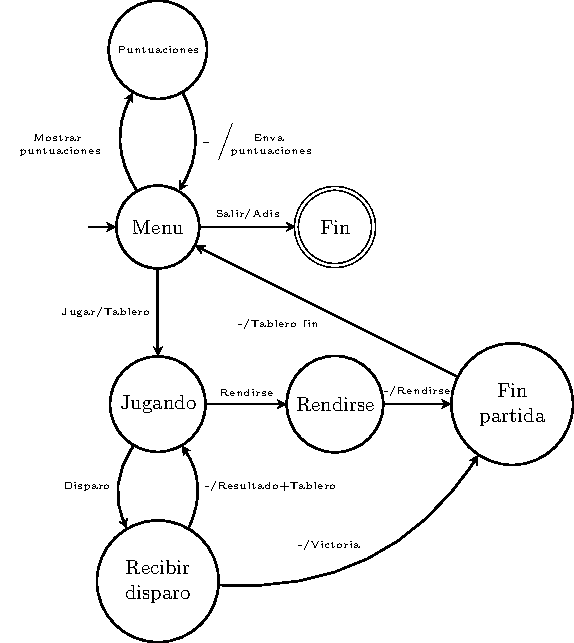
\includegraphics[width = 115mm]{estados_servidor}
\end{figure}

Los diferentes estados en los que puede encontrarse el servidor son los siguientes:

\begin{itemize}
\item \textbf{Menú:} Menú principal donde se muestran las diferentes opciones con la función \texttt{menu()} y se lee la opción elegida.
\item \textbf{Puntuaciones:} Se muestran las puntuaciones obtenidas en las partidas anteriores con la función \texttt{printPuntuaciones()}.
\item \textbf{Salir:} Envía un mensaje de ``Adiós'' y finaliza.
\item \textbf{Jugando:} Nos encontramos en medio de la partida. Podemos recibir disparos o rendición.
\item \textbf{Recibir disparo:} Con la función \texttt{receiveShot(x,y)} determinamos el resultado del disparo. En caso de victoria, finalizamos la partida.

\item \textbf{Rendirse:} Ponemos la puntuación a cero y finalizamos la partida.
\item \textbf{Fin de Partida:} Guardamos la puntuación y enviamos la localización de los barcos.
\end{itemize}

\section{Tipo de mensajes}

Hay dos tipos de códigos en nuestro programa: Las opciones del menú y los resultados del disparo.

\begin{itemize}
  
\item Opciones del menú. Son códigos de un sólo digito:
  \begin{enumerate}
  \item[1 -] Jugar una partida
  \item[2 -] Mostrar puntuaciones
  \item[3 -] Salir del juego
  \end{enumerate}

  Ante la opción del menú escogida, el servidor enviará el tablero (6 líneas), la lista de puntuaciones (2 líneas) o el mensaje de despedida (1 línea). Por lo tanto el número de líneas leidas por el cliente varían.
  
\item Resultados del disparo. Son códigos de dos dígitos:
  \begin{itemize}
  \item Códigos para fallos: Empiezan por 9.
    \begin{enumerate}
    \item[90 -] Agua: Has disparado a una casilla válida, pero no hay ningún barco.
    \item[91 -] Repetida: Ya has disparado a esa casilla.
    \item[92 -] Fuera: Te has salido del tablero.
    \item[99 -] Rendirse.
    \end{enumerate}

  \item Barco tocado: 1 seguido del nº del barco tocado (1,2,3).
  \item Barco hundido: 2 seguido del nº del barco tocado (1,2,3).
  \item Has ganado la partida: 33.
  \end{itemize}

  El cliente deberá seguir jugando, excepto si la partida termina. En cuyo caso el código de mensaje será 33 (victoria) o 99 (rendirse).
  
\end{itemize}

\section{Capturas de pantalla}

\begin{figure}[H]
  \centering
  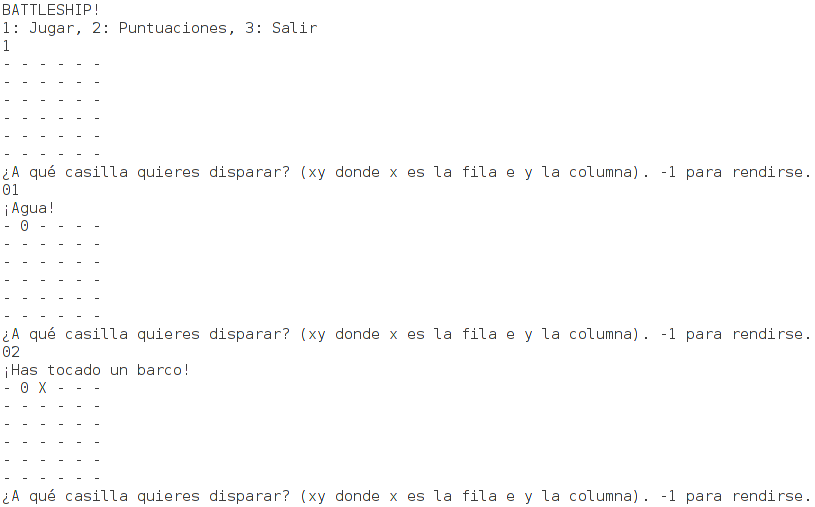
\includegraphics[width = 161mm]{imagenes/Inicio_juego}
  \caption{Iniciamos una partida, fallamos un disparo y acertamos otro. 0 : Agua, X : Barco, - : Desconocido}
\end{figure}

\begin{figure}[H]
  \centering
  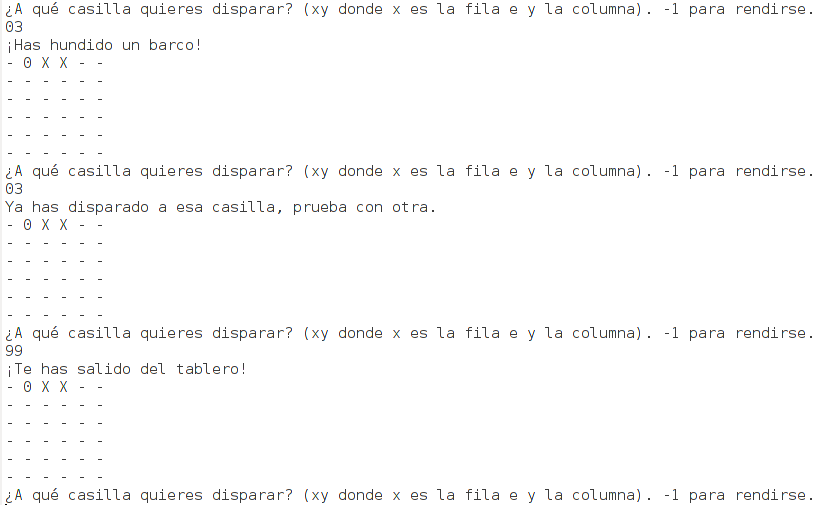
\includegraphics[width = 161mm]{imagenes/sigo_jugando}
  \caption{Hundimos el primer barco, disparamos en una casilla donde ya habíamos disparado y disparamos fuera del tablero.}
\end{figure}

\begin{figure}[H]
  \centering
  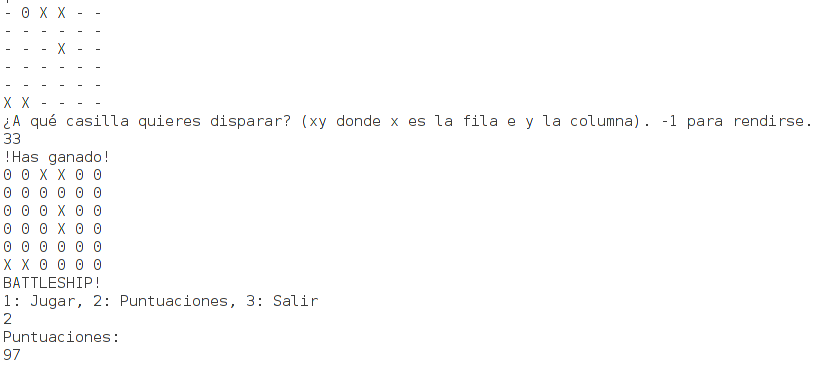
\includegraphics[width = 161mm]{imagenes/final}
  \caption{Ganamos la partida, nos muestra la localización de los barcos, nos envía el menú principal y vemos las puntuación de la partida.}
\end{figure}

\begin{figure}[H]
  \centering
  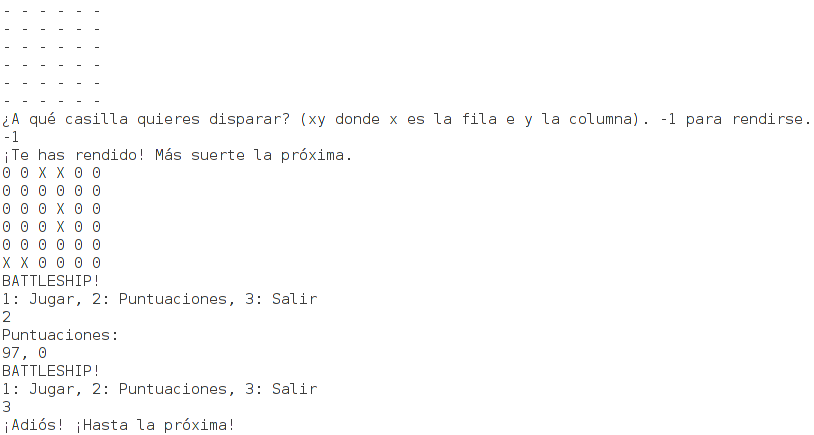
\includegraphics[width = 161mm]{imagenes/rendicion}
  \caption{Nos rendimos y nos muestra la localización de los barcos. Luego consultamos las puntuaciones obtenidas hasta el momento (97 puntos en la anterior partida y 0 en ésta). Después salimos del juego.}
\end{figure}

\end{document}